\def \nkois {8054}
\def \ncand {4034}
\def \newkois {738}
\def \newcand {219}
\def \completeness {85.21}
\def \reliability {97.14}
\def \effectiveness {99.6}
%For above numbers see script-playPublicData

\subsection{Summary of the KOI Catalog}

The final DR25 catalog, available at the NASA Exoplanet Archive contains all TCEs that pass the not-transit like tests (\S\ref{nottransitlikesec}). 


Some overall statistics of the DR25 KOI catalog are as follows:
\begin{itemize}
    \item \nkois{}~KOIs
    \item \ncand{}~PCs
    \item \newkois{}~new KOIs
    \item \newcand{}~ new PCs
    \item \completeness{}\% of \injtce{s} are PCs
    \item \effectiveness{}\% of \invtce{s} and \scrtce{s} are FPs
\end{itemize}

A summary of the planet radii and period of the planet candidates available in this catalog is shown in Figure~\ref{f:catalogPlot}. A clear excess of candidates exists with periods near 370\,d;  this excess disappears if we only consider those with a disposition score of 0.7 and greater. While the disposition score provides an easy way to make an additional cut on the PC population at long periods, when discussing the catalog PCs below we are using the pure dispositions of the Robovetter unless otherwise stated. The deficit of planets with radii just below 2.0\,R$_{\oplus}$ is consistent with the study of \citet{Fulton2017} where they report a natural gap in the abundance of planets between super-Earths and sub-Neptunes by applying precise stellar parameters to a subset of the \kepler\ transiting candidates \citep{CKS1,CKS2}. The new KOIs with a disposition of PC are found at all periods, but only 10 have MES$\geq 10 $. 

\begin{figure*}[ht]
    \centering
    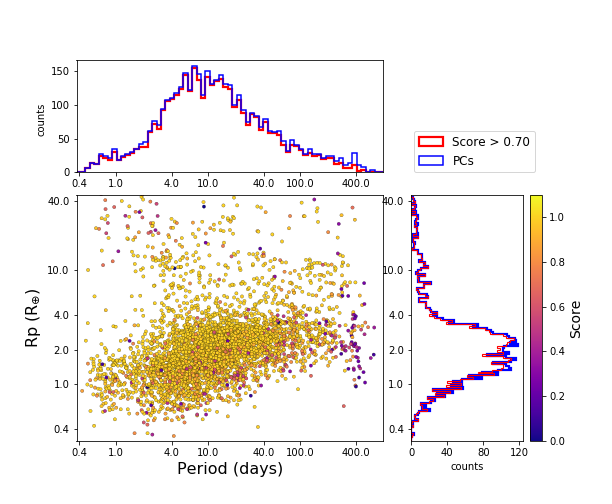
\includegraphics[width=1.1\linewidth]{fig-radiusPeriodScore-hist.png}
    \caption{DR25 planet candidates plotted as planet radius against period with the color representing the disposition score. The period and planet radii distributions are plotted on the top and on the left, respectively, in blue. The red line shows the distributions of those PCs with a disposition score greater than 0.7. The excess of PCs at long-periods disappears when cutting the population on disposition score. }
    \label{f:catalogPlot}
\end{figure*}

\subsection{Compare Dispositions to Other Catalogs}
We compare the catalog to two sets of \Kepler\ exoplanets: the confirmed exoplanets and the certified false positives.  In both of these cases, additional observations and careful vetting are used to verify the signal as either an exoplanet or a Certified False Positive \citep{Bryson2017c}. It is worth comparing the Robovetter to these catalogs as a sanity check.  

We use the confirmed exoplanet list from the Exoplanet Archive\footnote{https://exoplanetarchive.ipac.caltech.edu/cgi-bin/TblView/nph-tblView?app=ExoTbls\&config=planets} on 2017-05-24.  2279 confirmed planets are in the DR25 KOI catalog.  The DR25 Robovetter fails 44 confirmed planets, less than 2\%. Half of these FPs are not transit-like fails, 16 are stellar eclipse fails, six are centroid offsets and one is an ephemeris match. Twelve fail due to the LPP metric, all have periods less than 50 days.  The LPP metric threshold was set to improve the reliability of the long period KOIs, an act which sacrificed some of the short period KOIs.  The reason the Robovetter failed each confirmed planet is given in the ``koi\_comment" column at NExScI (see \S\ref{s:minorflags}). 

For the vast majority of the Robovetter FPs on the confirmed planet list, careful inspection reveals that there is no doubt that the Robovetter is incorrect. As an example, Kepler-10b \citep[][]{Batalha2011Kepler10,Fogtmann2014Kepler10}, a rocky planet in a 0.84~days orbit, was failed due to the LPP metric. This occurred because the detrending algorithm (the harmonic identification and removal algorithm in TPS, see \citet{JenkinsKDPH}) used by the \Kepler\ pipeline significantly distorts the shape of the transit, a known problem for strong, short period signals \citep{Christiansen2015} that the LPP metric ignores. 

In some cases the Robovetter may be giving the correct disposition.  Many of the confirmed planets are only statistically validated \citep{Morton2016,Rowe2014}. In these cases no additional data exists proving the existence of a planet outside of the transits observed by \Kepler. It is possible that the DR25 light curves and metrics have now revealed evidence that the periodic events are caused by noise or a binary star. For example, Kepler-367c \citep{Rowe2014}, Kepler-1507b \citep{Morton2016} and Kepler-1561b \citep{Morton2016}, (K02173.02, K3465.01 and K04169.01 respectively) were all confirmed by validation and have now failed the Robovetter because of the new ghost metric \S\ref{s:ghost}, indicating that the events are caused by a contaminating source not localized to the target star.  These validations should be revisited in the light of these new results.

{\color{blue}
It is also worth noting that none of the confirmed circumbinary planets \citep[e.g.,][]{Doyle2011,Orosz2012} are in the DR25 KOI catalog, however the binary stars that they orbit are listed as FPs.  The timing and shape of the circumbinary planet transits vary in a complicated manner, making them unsuitable for detection by the search algorithm used by the \Kepler{} Pipeline to generate the DR25 \opstce{} list.  As a result this catalog cannot be used for occurrence rate estimates of circumbinary planets, and their absence in the KOI catalog should not cast doubt on their veracity. 
}

% state what the accuracy of the statistical validation.

We use the Certified False Positive table\footnote{\url{https://exoplanetarchive.ipac.caltech.edu/cgi-bin/TblView/nph-tblView?app=ExoTbls\&config=fpwg}} downloaded from the Exoplanet Archive on 2017-07-11 to evaluate the performance of the Robovetter at removing known FPs. This table contains objects known to be FPs based on all available data, including ground-based follow-up information.  The Robovetter passes 106 of the 2713 certified false positives known at the time, only 3.9 per cent.  Most of those called PCs by the Robovetter are high signal-to-noise and more than half have periods less than 5 days.  The most common reason they are certified FPs is that there is evidence they are eclipsing binaries. In some cases, external information, like radial velocities provide a mass which determines that the KOI is actually a binary system. The other dominant reason for the discrepancy between tables is that the certified FPs often show evidence of significant centroid offsets. In crowded fields the Centroid Robovetter (\S\ref{s:centroidrv}) will not fail observed offsets because of the potential for confusion. For the Certified False Positive table, individual cases are examined by a team of Scientists who determines when there is sufficient proof that the signal is indeed caused by a background eclipsing binary.  

